\documentclass{article}


\usepackage[margin=1in]{geometry}
\usepackage{mathtools} %also loads amsmath
\usepackage{amssymb, bbm}
\usepackage[backend=biber,
	style=alphabetic,
	%	citestyle=authoryear,
	natbib=true,
	url=true, 
	doi=true]{biblatex}

%\usepackage{blkarray} % for matrices with labels
\usepackage{microtype}
\usepackage{relsize}
\usepackage{environ}% http://ctan.org/pkg/environ; for capturing body as a parameter for idxmats
\usepackage{tikz}
	\usetikzlibrary{positioning,fit,calc, decorations, arrows, shapes, shapes.geometric}
	\pgfdeclaredecoration{arrows}{draw}{
		\state{draw}[width=\pgfdecoratedinputsegmentlength]{%
			\path [every arrow subpath/.try] \pgfextra{%
				\pgfpathmoveto{\pgfpointdecoratedinputsegmentfirst}%
				\pgfpathlineto{\pgfpointdecoratedinputsegmentlast}%
			};
	}}
	%%%%%%%%%%%%
	
	\tikzset{dpadded/.style={rounded corners=2, inner sep=0.9em, draw, outer sep=0.4em, fill=gray, fill opacity=0.08, text opacity=1}}
	\tikzset{active/.style={fill=blue, fill opacity=0.1}}
	\tikzset{square/.style={regular polygon,regular polygon sides=4, rounded corners = 0}}
	\tikzset{octagon/.style={regular polygon,regular polygon sides=8, rounded corners = 0}}
	
	
	\tikzset{alternative/.style args={#1|#2|#3}{name=#1, circle, fill, inner sep=1pt,label={[name={lab-#1},gray!30!black]#3:\scriptsize #2}} }
	
	
	\tikzset{bpt/.style args={#1|#2}{alternative={#1|#2|above}} }
	\tikzset{tpt/.style args={#1|#2}{alternative={#1|#2|below}} }
	\tikzset{pt/.style args={#1}{alternative={#1|#1|above}} }
	

	\tikzset{mpt/.style args={#1|#2}{name=#1, circle, fill, inner sep=1pt,label={[name={lab-#1},gray]\scriptsize #2}} }
	\tikzset{pt/.style args={#1}{name=#1, circle, fill, inner sep=1pt,label={[name={lab-#1},gray]\scriptsize #1}} }
	
		
		 %\foreach \x in {#1}{(\x) (lab-\x) } 
		 
	\tikzset{Dom/.style args={#1 (#2) around #3}{dpadded, name=#2, label={[name={lab-#2}] #1}, fit={ #3 } }}
	\tikzset{Dom/.style args={#1 (#2) around #3}{dpadded, name=#2, label={[name={lab-#2}] #1}, fit={ #3 } }}
	\tikzset{bDom/.style args={#1 (#2) around #3}{dpadded, name=#2, label={[name={lab-#2}]below:#1}, fit={ #3 } }}
	\tikzset{arr/.style={draw, ->, thick, shorten <=3pt, shorten >=3pt}}
	\tikzset{archain/.style args={#1}{arr, every arrow subpath/.style={draw,arr, #1}, decoration=arrows, decorate}}
	%\tikzset{every label/.append style={text=red, font=\scriptsize}}
	
%	\newcommand\tikzdom[#1;#2](#3,#4[#5]){
%		\foreach [evaluate=\x as \y using (\x-#2/2)/#5 + #3] \x in {0, 1, ..., #2} {
%			\node[bpt={#1\x | $\n_\x$}] at (\y,#4) {};
%		}
%		\node[Dom={$\sf W$ (W) around \lab{w1}\lab{w3}}] {};
%	}

\usepackage{color}
\definecolor{deepgreen}{rgb}{0,0.5,0}

\usepackage[colorlinks=true, citecolor=deepgreen]{hyperref}


\setlength{\skip\footins}{1cm}
\setlength{\footnotesep}{0.4cm}

\usepackage{parskip}
\usepackage{amsthm, thmtools}
\usepackage{
	nameref,%\nameref
	hyperref,%\autoref
	% n.b. \Autoref is defined by thmtools
	cleveref,% \cref
	% n.b. cleveref after! hyperref
}

\begingroup
\makeatletter
\@for\theoremstyle:=definition,remark,plain\do{%
	\expandafter\g@addto@macro\csname th@\theoremstyle\endcsname{%
		\addtolength\thm@preskip\parskip
	}%
}
\endgroup
\makeatother

\theoremstyle{plain}
\newtheorem{theorem}{Theorem}[section]
\newtheorem{coro}{Corollary}[theorem]
\newtheorem{prop}[theorem]{Proposition}
\newtheorem{lemma}[theorem]{Lemma}
\newtheorem{fact}[theorem]{Fact}
\newtheorem{conj}[theorem]{Conjecture}

\theoremstyle{definition}
\newtheorem{defn}{Definition}[section]
\newtheorem{examplex}{Example}[section]
\newenvironment{example}
	{\pushQED{\qed}\renewcommand{\qedsymbol}{$\triangle$}\examplex}
	{\popQED\endexamplex\vspace{-1em}\rule{1cm}{0.7pt}\vspace{0.5em}}

\theoremstyle{remark}
\newtheorem*{remark}{Remark}

\usepackage{xstring}
\usepackage{enumitem}

%\newcommand\duplicat[1]{\gdef\mylist{}\foreach \x in {#1}{\xdef\mylist{\mylist (\x) (lab-\x) }}\mylist} %% this doesn't work :((
\newcommand\lab[1]{(#1)(lab-#1)}


\newcommand{\todo}[1]{{\color{red}\large\textbf{[todo}: {\normalsize\itshape#1}\textbf{]}}}
\newcommand\geqc{\succcurlyeq}
\newcommand\leqc{\preccurlyeq}
\newcommand\mat[1]{\mathbf #1}
\newcommand{\indi}[1]{\mathbbm{1}_{\left[\vphantom{\big[}#1 \vphantom{\big]}\right]}}
\newcommand\m[1]{\mathbf m_{\mathsf #1}}

\newcommand\recall[1]{ Recall \expandarg\cref{rex:#1}:\vspace{-1em} \begingroup\small\color{gray!80!black}\begin{quotation} \expandafter\csname rex:#1\endcsname* \end{quotation}\endgroup }

%OMG THIS WORKS

\def\wrapwith#1[#2;#3]{
	\expandafter#2{\expandarg\StrBefore{#1}{,}}
	\expandarg\StrBehind{#1}{,}[\tmp] 
	\xdef\tmp{\expandafter\unexpanded\expandafter{\tmp}}
	#3
	\expandarg\IfSubStr{\tmp}{,}{\wrapwith{\tmp}[#2;{#3}]}{ \expandafter#2{\tmp} }
}
\def\hwrapcells#1[#2]{\wrapwith#1[#2;&]}
\def\vwrapcells#1[#2]{\wrapwith#1[#2;\\]}



\newsavebox{\idxmatsavebox}
\def\makeinvisibleidxstyle#1#2{\phantom{\hbox{#1#2}}}
\newenvironment{idxmat}[3][\footnotesize\color{gray}\text]{%
	\def\idxstyle{#1}
	\def\colitems{#3}
	\def\rowitems{#2}
	\begin{lrbox}{\idxmatsavebox}$
	\begin{matrix}  \begin{matrix} \hwrapcells{\colitems}[\idxstyle]  \end{matrix} \\[0.1em]
		\left[ 
		\begin{matrix}
			\hwrapcells{\colitems}[\expandafter\makeinvisibleidxstyle\idxstyle]  \\[-1em]
	}{
		\end{matrix}\right]		&\hspace{-0.5em}\begin{matrix*}[l] \vwrapcells{\rowitems}[\idxstyle] \end{matrix*}
	\end{matrix}
	$\end{lrbox}
	\raisebox{0.75em}{\usebox\idxmatsavebox}
%	\vspace{-0.5em}
}

\newenvironment{sqidxmat}[2][\footnotesize\color{gray}\text]
	{\begingroup\idxmat[#1]{#2}{#2}}
	{\endidxmat\endgroup}
\usetikzlibrary{cd}

\usepackage{ wasysym }


\addbibresource{../refs.bib}
\addbibresource{../maths.bib}


\newcommand{\mfem}{\mathclap\female\male}
\newsavebox{\hourglassbox}
\savebox{\hourglassbox}{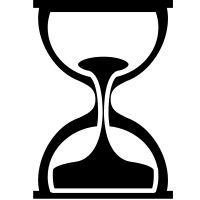
\includegraphics[height=.8em]{hourglass.png}}
\newcommand\hourglass{\usebox{\hourglassbox}}

\title{Discussion of \todo{need name for model} Semantics and Consistency}
\author{Oliver Richardson  \texttt{oli@cs.cornell.edu}}

\newcommand\modelname{{\color{green!50!black}$\langle$model name$\rangle$ }}

\begin{document}
	\maketitle

%	\section{The problem with expressing impact as conditional probability.}
%	
%	When we say we have a domain of ``goodness'' $\sf U$, and a conditional probability distribution $\Pr(U \mid A)$, we are not expressing the goodness of $A$, rather estimating the goodness of the world where $A$ takes on various values. This is obviously a belief, and does not work as an expected utility calculation.  How to fix?
%	
%	\subsection{Add more nodes: a separate node for each component}
%	\subsection{Change impact arrows to be functions.}


%	Suppose that we have a diagram
%	
%	\begin{tikzpicture}
%		\node[dpadded](X){$X$};
%		\node[dpadded](A) at (-1, -1.3) {$A$};
%		\node[dpadded](B) at (1, -1.3) {$B$};
%		\node[dpadded](U) at (0, -2.6) {$U$};
%	\end{tikzpicture}

%	Goal: learn preferences over variables, which changes as slowly as possible, to be used in prediction. The classical picture of decision theory is a limit point with infinite cognitive power. You have to coordinate the different levels of preferences, and be very careful to avoid conflicts. 

%	\section{A Defense of  Semantics.}
	Recall that we have a model of nodes, chained together with Markov kernels / conditional probability distributions / stochastic matrices. Of course, there is already an enormous literature about diagrams which look somewhat like this, made up of nodes and conditional probability tables: Baysian Networks (BNs) and their many variants. The diagrams that we employ look very similar, but are intended for a different purpose, and hence have a different semantics. Whereas BN's are a factorization of a particular joint probability distribution and consistent by design, these models are merely constraints on the distribution, which might be so strong so as not to admit any joint distribution.
	
	We will go into the difference more carefully in the next section, but first here are some reasons to prefer this as a way of modeling agents,% in the order of explanation rather than importance:
	
	\begin{enumerate}[nosep]
		\item This representation more naturally matches what humans are aware of, encoding small locally consistent models rather than one giant probability distribution.
		\item It is cleaner from a mathematical standpoint: utilities and probabilities are related, we get a notion of belief composition, and we can make use of both category and information theory.
		\item This allows composition of arrows to be defined, and gives meanings to paths. 
		\item When bits of these diagrams are added and removed, the meaning and form of the rest of the diagram remains the same.
		\item We can now represent inconsistency, which we will use to drive preference change. While we agree with the classical picture in that inconsistency is bad, now we can talk about it. 

		\item Due to the compositionality, it is possible to add typing rules to dynamically change beliefs, knowledge representations, and so forth (section \ref{sec:belief-typing})
		\item It is a strictly more general representation--- we can easily convert BNs to these diagrams (section \ref{sec:convert2bn})
	\end{enumerate}

	\subsection*{Recap: \modelname Definitions and Semantics}
	\begin{defn}
		A \modelname model $(\cal A, L)$ is a collection of variables $\cal A$, attached to each of which is some preference information: (this could be an order, utility, pairwise utility matrix, a supremum function), plus a collection of probabilistic links $\cal L$ between some (but not necessarily all) pairs of them, where $L: A\to B \in \cal L$ is a (sub) Markov kernel $A \to \Delta (B \cup \{\bullet\})$\footnote{The additional ``phantom element'' $\bullet$ absorbs probability density that we don't want to equivocate on, allowing our model to capture partial families of conditional probabilities, by extension things like implication, and giving agents more tools to avoid inconsistency. This has the effect of making our links substochatic matrices/kernels rather than stochastic ones. However, if we restrict to beliefs which assign zero probability to $\bullet$, everything in the model works as before.} representing beliefs about how a setting of $A$ will impact the value of $B$. 
	\end{defn}

	
	
	In this document, we will focus on models where the preference information is encoded as a special utility domain $U$, with links from other variables. While there may be some propositions tying this case to utilities or preference orders, we will avoid talking explicitly about the more general setting of preference matrices and choice functions out for now.
	
	
	\section{Defense of \modelname Models}
	\subsection{The Possibility of Type Constructors}\label{sec:belief-typing}
	The classical picture also features a fixed set of variables. In addition to allowing new concepts to form, we would like to have inductive ways of introducing new ones logically, as combinations of the existing variables. Interpreting variables as types, whose possible assignments are terms, the syntax of which variables we can construct and what beliefs we have about the resulting picture is a type theory. There are some obvious ways one might want to combine existing domains; the one we are concerned with here is products.
	
	In terms of beliefs, you might already have beliefs about how likely two  $A$ and $B$, then suddenly wonder about how they interact. For instance, you may already have beliefs about how likely you are to leave your keys in the ignition, and also how often your car is dead, and then wonder if there's a connection. 
	In terms of preferences, you might think $a \geqc a'$ and $b \geqc b'$, but now wonder what you would do if you had to choose between $a b'$ and $a' b$. In both cases, you are slightly enlarging your picture to consider the relevant features that a classical agent would already have.
	
	For this reason, we introduce the possibility of creating a domain $A \times B$, if $A$ and $B$ are nodes in the picture, whose elements are the cartesian product of $A$ and $B$. Moreover, this comes with projection links $\pi_A : A \times B \to \Delta(A)$, $\pi_B: A\times B \to \Delta B$ given by $\pi_A((a,b), a') = \delta_{a,a'}$ and $\pi_B((a,b), b') = \delta_{b,b'}$, as usual. Furthermore, we can construct a function $\langle f , g \rangle : X \to A \times B$ for any $f: X \to A$ and $g: X \to B$ that make the picture no more inconsistent.
	This is represented graphically as the usual product diagram:
	\begin{center}
		\begin{tikzcd}
			&X\ar[dl,"f"']\ar[dr,"g"]\ar[d, "{\langle f, g \rangle}"description ]  \\
			A & A \times B \ar[l, "\pi_A"]\ar[r, "\pi_B"'] & B
		\end{tikzcd}
	\end{center}
	
	It may be worth noting that we can always construct $\langle f, g \rangle$, but uniqueness in general does not hold, so it is not (yet) a categorical product.
	
	\subsubsection{Products vs Unions}
	
	We could have achieved a similar thing by considering $\{A\}$ and $\{B\}$ as singleton sets of variables, and then adding $\{A,B\}$ to the picture. Here we would interpret as a set of random variable taking values in the range of the product of its elements possible values. The two accounts differ when there is an overlap between the sets. Should we be allowed to represent $A \times A$? 
	
	Taking unions does protect us from doing certain bad things: it would be a mistake to assign a distribution $\Pr(a, a') > 0$ for $ a \neq a'$, for instance --- but we're already in the business of allowing this kind of inconsistency --- in the picture below all the marginals are fine as far as the syntax is concerned, but there is no way to assign a probability distribution on all of the nodes.
	\begin{center}
		\begin{tikzcd}
			&1 \ar[d, "p(A\times A)"] \\
			 & A \times A \ar[ld]\ar[rd] & \\
			 A \ar[rr,equal]&& A
		\end{tikzcd}
	\end{center}

	It can also be very useful to keep extra copies of $A$ around even if (part of) one already exists buried in another variable, because we can delay integration using this trick, as in example \ref{ex:bayesrule} for instance. The most compelling reason for me is that one might not know that you're looking at two copies of $A$; maybe they've been framed differently --- but still you should be able to take a product and get two things, rather than a union, which immediately leaks the truth of their equivalence to an agent.
	
	
	
	% Motivating example: why do we need A x B?  Why not just have a BN?
	%	If $A$ and $B$ are random variables, 
	
	
	
	
	
	\subsection{Converting BNs}\label{sec:convert2bn}
	The semantics of a Baysian network ensure that there is no inconsistency: the arrows into a node taken together collectively determine the correct probability distribution. We have a collection of nodes $\cal N$, and for each $N \in \cal N$, we have a set of parents $\mathrm{Par}(N)$, and a conditional probability distribution $\Pr( N \mid \mathrm{Par}(N))$, which is a distribution over the values of $N$ for each setting of every variable in $\mathrm{Par}(N)$. Note that each of our arrows carries a meaning by itself, a collection of arrows into a single node must be taken together to have any meaning in a BN. 
	
	The procedure for converting to a BN is simple: we simply take every node's incoming arrows, and insert the product of its parents as a node before it. With this procedure, if a node $N$ has just one parent $P$, we replace $P \to N$ with $P \to N ~=~ N$, which is redundant so we don't draw this. If a node had zero parents (i.e., the BN just gives it a probability distribution not dependent on anything), we insert the product of zero things, i.e., the singleton node $1 = \{*\}$, a variable which only takes one value, and set $\Pr(N \mid *) = \Pr(N)$. 
	
	This sound much more complicated than it is. Consider the example below, where the left is a BN, and the right is the corresponding \modelname.
	\begin{center}
		
		\begin{tikzcd}[baseline={([yshift=-.8ex]current bounding box.center)}, column sep=2.5em]
			& A \ar[dl]\ar[dr] \\
			B \ar[dr] && C \ar[dl]\\
			& D &
		\end{tikzcd}
		\hfil
		\begin{tikzcd}[baseline={([yshift=-.8ex]current bounding box.center)}, column sep=2em]
			& \mathsf 1 \ar[d] &\\
			& A \ar[dl]\ar[dr] \ar[dd,dashed, gray] \\
			B && C \\
			& B \times C \ar[ul, gray!70] \ar[ur, gray!70]\ar[d] & \\
			& D &
		\end{tikzcd}
	\end{center}
	\vspace{0.5em}

	We have effectively changed two things: first, visually encoded the probability distribution of $A$ as the arrow $1 \to A$ (which we are now allowed to omit; sometimes you don't want priors on things, such as your own actions). Second, we have combined the two arrows $B \to D$ and $C \to D$ into a single one, $B \times C \to D$. Though certainly more verbose, this is arguably visually clearer if want to follow arrows: you cannot compute $D$ from $B$; you need both $B$ and $C$.
	
	% The BN makes the assumption that the value of $D$ cannot depend on anything else; we're only 
%	This also illustrates another important point: the assumptions that you make to drawn a BN, even if locally sensible, build on one another and might not end up being what you wanted to model. On the left it visually looks like you can estimate $D$ from $B$, which is false. It also looks like you can estimate $D$ from $A$ --- which is true, but only if we've actually modeled all of the confounding factors! For instance, if $B$ has some small mostly negligible dependence on another variable $E$, then maybe the $A \to B$ link works out with very little error, but 
	
	\subsection{Human Preferences}
	\begin{example}
		After reading a number of empirical studies, you come to believe that smokers have a 70\% chance of developing cancer, compared to 20\% for non-smokers. At the same time, you believe that those who use tanning beds have a 80\% chance of developing cancer, compared to 18 \% for those who do not use them. You have no information about how the two interact.
	\end{example}
	
	\begin{example}
		You are on a game show, and offered a choice between several levers $(A)$; your choice will determine how much money you receive. You are uncertain what each lever does, but you do have a vague intuition about the mechanism, giving you a distribution over amounts for each lever ($\Pr(C \mid A)$). You also had enough time to read statistics about how well people have done in the past $(\Pr(C))$. You do not have any information about what levers they've chosen though, nor do you have a complete joint probability $\Pr(A, C)$. 
		
		Still, there is a possibility
	\end{example}


	\subsection{Composition Of Arrows}
	\todo{Reword}
	This is necessary for composition to be defined for individual arrows. Since arrows are Markov kernels / matrices, composition is given in the usual way, by integration / summation over the intermediate variable --- if $f : A \times B \to \mathbb R$ and $g : B \times C \to \mathbb R$ (this is the finite case) we can obtain a stochastic matrix
	
	\[ g\circ f : A \times C \to \mathbb R =  \sum_{b \in B} f( b \mid a) g(c \mid b) \]
	
	For Markov chains, the state of $B$ entirely determines the state of $C$, and so if $f = p(B \mid A)$ and $g = p(C \mid B)$, $g\circ f = p(C \mid A)$. In our case, we also have the possibility of branching and merging. Let's now consider what it means for us to have a diagram 
	\begin{tikzcd}
		A \ar[r] & C & \ar[l] B
	\end{tikzcd}.
	This means an agent has probability distributions $\Pr(C\mid A)$ and $\Pr(C \mid B)$%
	% (again, as opposed to the BN interpretation, which would be a single distribution $p(C \mid A, B)$)%
	. Often, this is a perfectly coherent picture, and is in fact the kind of data people actually have:
	


	However, this information may not be entirely complete, feel strange, be contradictory, or make it seem as though the choice is an illusion. This ``outside view'' is also important for constructing Newcomb's problem:
	
	\begin{example}[Newcomb]
		There are two boxes. Box 1 is clear and visibly contains \$1k; box 2 is opaque, and will contain \$1M if a predictor (which you know has been very accurate in the past) predicts you will leave box 1, and nothing if it predicts you will take both.
		Now, you have a probability distribution of money based on predicted actions $\Pr(\$ \mid P)$, and also a causal mechanism that predicts the amount of money given your current actions $\Pr(\$ \mid A)$
		\begin{center}
			\begin{tikzcd}
				A \ar[rd] &  & \ar[ld] P \\ & \$
			\end{tikzcd}
		\end{center}
		More weirdness comes from the fact that $A$ and $P$ interact.
	\end{example}

	\section{Composition of Stochastic Links}


	
	
	\subsection{Should paths be equal?}
	
	This design decision also has the effect of proving multiple ways to calculate things, which leads to the somewhat counter-intuitive fact that that not all diagrams commute, even ignoring preferences entirely. We will begin by explaining why this might not be what one would expect. If the model is acyclic, every diagram (trivially) commutes, and even in our setting, many probability axioms require commuting diagrams.
	
	\begin{example}[Marginalization]
		Recall how a probability can be obtained by marginalization:
		\[ p(b) = {\color{gray}\sum_{a \in A} p(a \land b) = \sum_{a \in A} p(a) \frac{p(a\land b)}{p(a)} }= \sum_{a \in A} p(a) p(b\mid a) \]
		below is an illustration of this fact:
		\begin{center}
			\begin{tikzcd}
				& 1 \ar[ld, "\Pr(A)"']\ar[rd, "\Pr(B)"] \\
				A \ar[rr]\ar[rr,"\Pr(B \mid A)"'] &  & B\\
			\end{tikzcd}
		\end{center}
		The left part of the diagram represents the right side of the equation and vice versa. 
	\end{example} 

	This can be used inductively to show that every pair of paths from the singleton object $1$ is equivalent, but before that we will deal with another important case:
	
	\begin{example}[Bayes Rule] \label{ex:bayesrule}
		We can also represent Bayes' rule, $p(a \mid b) p(b) = p(b \mid a) p(a)$ as an assertion that two paths from:
		\begin{center}
			\begin{tikzcd}
				&1 \ar[dl, "\Pr(A)"']\ar[dr,"\Pr(B)"]\\
				A \ar[dr, "\Pr(B \times A \mid A)"'] & & B  \ar[dl, "\Pr(B \times A \mid B)"]\\
				& B \times A 
			\end{tikzcd}
		\end{center}
		This can be seen as two applications of marginalization, one for each half. On the left, we have
		\[ p(b, a) = \sum_{a' \in A} p(a')p(a,b \mid a') = \sum_{a' \in A} p(a') p(b \mid a') \delta_{a,a'} = p(a) p(b \mid a) \]
		and similarly, the right gives $p(b,a) = p(b) p(a \mid b)$. One thing to take away is that one can avoid the integration over a variable by simply considering the conditional distribution to a different variable: namely, one which is the product of the input and output. 
	\end{example}
	
	
	However, not all paths generated by composition of probabilities are strictly equal! In an extreme case, we can forget all of our information with the Markov assumption by going through a singleton object:
	
	\begin{center}
		\begin{tikzcd}
			A \ar[rd]\ar[rr,"\Pr(A\mid A) = \mathrm{id}_A"] &  & A\\&1 \ar[ru, "\Pr(A)"']
		\end{tikzcd}
	\end{center}
	For this to happen, the only thing we need is to allow composition and provide a probability on $A$; there's nothing inconsistent about this picture. Therefore, the measure of consistency is weaker than ``all paths are equal''. Still, there are some blatantly inconsistent pictures one could draw --- anything that violates Bayes' rule or marginalization, for example (see section \ref{sec:inconsistency-ex} for more).
	
	Our singleton example is a little bit annoying, but at least it's the best prediction that could be made after forgetting all of the information. It is natural to ask: can composition of conditional probabilities do \emph{worse} than ignoring everything? Or is every bit of signal helpful? % There are two competing intuitions here: on the one hand, correlations are not transitive; on the other, if an intermediate variable $Y$ is positi
	
	\begin{example}
		Men earn more than women, and people who earn more are generally older, but women live longer than men, so the top composition in the picture below
		\[ \begin{tikzcd}
			& \$ \ar[rd] \\Types
			\mfem \ar[rr]\ar[ru] &&  \hourglass
		\end{tikzcd} \]
		is worse than ignoring all information and just predicting age. Here it is with numbers. Suppose the truth is a conditional probability distribution $\Pr(\$, \hourglass \mid\mfem)$ given by
		
		\begin{center}
		\begin{tabular}{r|ccccc|}
			\multicolumn{1}{c}{}&\multicolumn{2}{c}{\male}  &&\multicolumn{2}{c}{\female} \\
			&$<$40 yr & $\geq$40 yr &\vline& $<$40 yr & $\geq$40 yr \\\cline{2-6}
			$<\$40$k & .225 & .05 && .185 & .19 \\
			$\geq\$40$k & .075 & .15 && .065 & .06\\\cline{2-6}
		\end{tabular}
		\end{center}
		We can now construct our chain, $\mfem \to \$ \to \hourglass$
		\begin{center}
		\begin{tikzcd}[column sep=1.5cm,row sep=1.2cm]
			m \ar[r, ".55"]\ar[rd, ".45"description,pos=0.8] & <\$40k \ar[r,".63"]\ar[rd,".37"description,pos=0.8] & < \text{40 yr} \\
			f \ar[r, ".25"']\ar[ru, ".75"description,pos=0.8] & \geq \$40k \ar[r,".60"']\ar[ru, ".40"description,pos=0.8] & \geq \text{40 yr}
		\end{tikzcd}
		\end{center}
		Now, consider the following three arrows $\mfem \to \hourglass$, as estimates of $\Pr(\hourglass \mid \mfem)$:\\
		
		\begin{minipage}{.33\linewidth}\centering
			(1) the truth, $\Pr(\hourglass \mid \mfem)$:\\[1em]
			\begin{tabular}{c|cc}\hline
				& $<$40 yr & $\geq$40 yr \\\hline
				\male & .6 & .4 \\
				\female & .5 & .5 \\\hline
			\end{tabular}
		\end{minipage}
		\begin{minipage}{.33\linewidth}\centering
			(2) $\mfem\to 1\to \hourglass$:\\[1em]
			\begin{tabular}{c|cc}\hline
				& $<$40 yr & $\geq$40 yr \\\hline
				\male & .55 & .45 \\
				\female & .55 & .45 \\\hline
			\end{tabular}
		\end{minipage}
		\begin{minipage}{.33\linewidth}\centering
			(3) $\mfem\to \$\to \hourglass$:\\[1em]
			\begin{tabular}{c|cc}\hline
				& $<$40 yr & $\geq$40 yr \\\hline
				\male & .53 & .47 \\
				\female & .57 & .43 \\\hline
			\end{tabular}
		\end{minipage}
		\vspace{1em}
		
		We can see that $(2)$, which kills all signal, is closer to the truth than (3) in every way. Still, the picture is entirely consistent. Moreover, all of the important details of the joint distribution are saved in the three arrows, and subjectively, I used the arrows to construct the joint distribution I wanted, rather than the other way around.
		
		Even though this triangle does not commute, still every pair of paths from $1$ to another node are equivalent; for instance, marginalizing out gender gives the same distribution on age in all three of the cases above.
	\end{example}

	\subsection{Some Results}
	Still, path equality is often expected; we would like to characterize when and why. Below are some necessary conditions for consistency, although more exploration is required.
	
	\begin{prop}\label{prop:prob-eq}
		If $\pi$ is a path of conditional probabilities $1 = A_0 \to A_1\to\cdots \to A_N = X$, then the composition $\pi^\circ$ of links in $\pi$ is equal to $\Pr(X)$.
	\end{prop}

	Similarly, we have the dual result for deterministic functions:
	\begin{prop}\label{prop:det-eq}
		If a variable $Q$ is completely determined by both $A$ and $B$, i.e., $g : A\to Q$ and $h : B\to Q$ are deterministic, and $f : A \to \Delta B$ is $\Pr(B \mid A)$, then $h \circ f = g$. 
	\end{prop}
	\begin{proof}
		If there is a non-zero probability that $A = a$ while $B = b$, then it must be the case that $g(a) = h(b)$, since both $a$ and $b$ determine $Q$. So
		\begin{align*}
			h \circ f(a,q) = \sum_{b \in B} f(a,b) \delta_{h(b),q}	
					= \sum_{b \in B} f(a,b) \delta_{g(a), q} 
					= \delta_{g(a),q} \sum_{b \in B} f(a,b) 
					= \delta_{g(a),q} 
					= g(a, q)
		\end{align*}
	\end{proof}

	To summarize: we have a picture containing conditional distriTypesbutions, particularly the ones which are most useful and actionable. Each conditional is a constraint on the world. We have a natural way of composing distributions, but sometimes the composition of two distributions is not the true probability.
	%Question: why even bother with composition, then? Why not just have arbitrary constriants?
	% Answer (1): composition does the right thing under markov assumption, and we can always move the representation in such a way that we can get a markov assumption.
	% Answer (2): If you have no other option this is the only estimate you have.
	% Answer (3): Up to the entropic cone, it is still guaranteed to be accurate.
	
	\section{Inconsistency}
	% This is a predicate definition. We would also like to have a continuous definition so we can do gradient descent. 
		
	\begin{defn}[consistency]
		A model $(\cal A, L)$ is \emph{consistent} if there exists some joint probability $\Pr(\cal A)$ on all of the variables, that is consistent with every link marginal $L \in \cal L$.
	\end{defn}


	\begin{defn}
		A model $(\cal A, L)$, in which preferences are represented by a single utility node $U \in \cal A$, is \textit{pref-inconsistent} if it is inconsistent, but only because of the utility node --- i.e., the model obtained by deleting $U$ and all links to it, $\big(\mathcal A \setminus U,~~\mathcal L \setminus \{ L : \square\to U \}\big)$ is consistent.
	\end{defn}

	To get readers on board with these definitions, we will show how they correspond to other intuitions of inconsistent preferences through some examples and specific cases
	
	\subsection{Intransitivity of Preferences as Inconsistency}
	

%	\begin{defn}
%		More generally, a model $(\cal A, L)$ is \emph{pref-inconsistent} 
%	\end{defn}


%	The thing that makes a picture inconsistent is an inability to assign any joint probability that marginalizes out to the conditional ones. %However, it is not clear how to make this differentiable. Perhaps minimizing inconsistency by using the previous sum-of-paths technique while it is inconsistent is important.
	
	\subsection{Examples of Inconsistency}\label{sec:inconsistency-ex}
	% Also, in some sense, the picture above is somehow the worst one could do by composition:
	\subsubsection{A short list}
	\begin{itemize}[nosep]
		\item Violations of either propositions \ref{prop:prob-eq} or \ref{prop:det-eq}
		\item Failure to obey entropy triangle inequality
		\item Outside of entropic cone.
	\end{itemize}

	\subsubsection{Belief Revision}
	
	\subsubsection{Framing Problems}
	\subsubsection{Learning Problems}
	
	\subsection{Sufficient Conditions for Inconsistency}
	\begin{prop}
		
	\end{prop}
\end{document}